\documentclass[12pt, a4paper]{article}

\usepackage{setspace, graphicx, lineno, caption, color, float}
\usepackage{amsmath}
\usepackage{amsfonts}
\usepackage{amssymb}
\usepackage{amsthm}
\usepackage{amstext} %to enter text in mathematical formulae
\usepackage{algpseudocode}%psuedo code and 
\usepackage{algorithm}%puts the psuedo code in a float box
\usepackage[retainorgcmds]{IEEEtrantools}
\usepackage{natbib}
%\usepackage{url, hyperref, makeidx, fancyhdr, booktabs, palatino}
%\usepackage{euscript} %EuScript, command: \EuScript, for letters in Euler script
%\usepackage{paralist} %listing (i), (ii), etc.
\usepackage{rotating} %rotating text
\usepackage{multirow} %connecting columns in tables
\usepackage{multicol}
\usepackage{longtable}
%image stuff
%\usepackage{epstopdf}
%\usepackage{cancel}
%\usepackage[ngerman, english]{babel} %for different languages in one document
%\usepackage[utf8]{inputenc}
%\hypersetup{colorlinks=true, linkcolor=blue}
%page set up

\usepackage[left=2.5cm,top=2.5cm,right=2.5cm, bottom=2.5cm,nohead]{geometry}
\doublespacing
%paragraph formatting
\setlength{\parskip}{12pt}
\setlength{\parindent}{0cm}

\begin{document}
Title: Optimal control in the face of evolving resistance by hiding portions of the population from selection.
Shaun R. Coutts, Dylan Z. Childs, ...

\section*{Introduction}
Controlling populations in the face evolving resistance to xenobiotics (i.e. antibiotics, herbicides, pesticides, fungicides) is one of the biggest challenges facing public health [REF], and food security [REF]. Evolved resistance costs many dollars globally [REFs, inc Audit paper], but this cost could be reduced with more responsive control strategies that take account of evolving resistance.

Finding optimal solutions over time is a challenging task due to time and order dependence, combinatorial optimization, particularly with a dynamic system. Decision theory sets out a series of steps to arrive at good decisions i) define the objective (in this case minimize discounted economic cost, minimize the weed population for a fixed budget) and encode that objective in a mathematical function (the reward function), ii) define the set of actions, iii) define a model that links each action to the objective function, iv) find the action that maximizes the reward function.

practical difficulties of this for resistance.           

There are proposed strategies for TSR [REX REF], which follow Mendelian inheritance, however something about quantitative resistance and potential for cross resistance. As a result strategies that work for TSR may not work for quantitative resistance.

Something about integrated weed management to reduce use of herbicides, and thus slow the development of resistance [Audit paper REF].      

We develop a model of quantitative resistance to two herbicides in an important weed of wheat in Europe. We embed this model in a decision theory framework to find good integrated weed strategies to manage a population where herbicide resistance can evolve, and there is potential cross resistance.        

\section*{Methods}
The purpose of the population model is to translate actions to the reward function. In this case we are modelling the population of black grass over time, its response to management actions and its impacts on wheat yield. We model a population that can become resistant to herbicide through evolved target site resistance. A commonly recommended [REX] and applied [Hicks et al] strategy to combat resistance and manage populations in the face of resistance is to apply herbicides that impair different cellar pathways (i.e. modes of action), either sequentially (cycling) or concurrently (stacking). To allow this behaviour in the optimal strategies we model two independent target site resistant genotypes in the same population.

We track the number of seeds in the seed bank with each resistance genotype ($g_1, g_2$) given action $a_q$ is taken. The action $a_q$ is how the manager effects the population model, and thus the reward they get from taking a given set of actions. Each action is a tuple of four sub-actions $a_q = \langle a_h, a_b, a_k, a_m \rangle$, see Appendix 1 for a description of the sub-actions and all the eligible combinations of these sub-actions (i.e. the full actions space, $\mathbf{A}$).   

\subsection*{Population model}
We use a discrete time, spatially implicit model, where herbicide resistance is assumed to be a quantitative, polygenic trait. We model the inheritance of resistance to both herbicides jointly, using the infinitesimal model [REF Fisher]. We model the black grass population using a yearly time step, starting at the beginning of the growing season before any seeds have emerged.

The seed bank at depth level $l \in \{1, 2\}$, time $t$, with resistance to herbicides 1 and 2 of $g_1$ and $g_2$ is 
\begin{subequations}
\label{eq:sb}
\begin{align}
	b(g_1, g_2, 1, t) &= b'(g_1, g_2, 1, t - 1)\phi_b (1 - \phi_e) + f(g_1, g_2, t-1)\\
	b(g_1, g_2, 2, t) &= b'(g_1, g_2, 2, t - 1)\phi_b	 
\end{align}      
\end{subequations} 
where $\phi_b$ is the proportion of seeds that survive from one year to the next, $\phi_e$ is the portion of seeds that germinate from the seed bank and $b'(g_1, g_2, l, t - 1)$ is the distribution of seeds over $g_1$ and $g_2$ at depth level $l$ in the previous year directly after plowing. To plow or not is the first management decision made (see Figure \ref{fig:life_cyc} for timing of management actions in the life cycle). Plowing moves seeds from one level of the seed bank to the other and is
\begin{subequations}
\label{eq:sb_pp}
\begin{align}
	b'(g_1, g_2, 1, t) &= b(g_1, g_2, 1, t) - b(g_1, g_2, 1, t) I a_b + b(g_1, g_2, 2, t) I a_b \\
	b'(g_1, g_2, 2, t) &= b(g_1, g_2, 2, t) - b(g_1, g_2, 2, t) I a_b + b(g_1, g_2, 1, t) I a_b
\end{align}
\end{subequations} 
where sub-action $a_b \in \{0, 1\}$ indicates if plowing was carried out or not and $I \in [0, 1]$ is the portion of seeds inverted to the other seed bank depth if plowing is carried out. The life cycle is closed by adding the seeds produced in the previous year ($f(g_1, g_2, t - 1)$) to the top layer of the seed bank in the current year.

To get the distribution of seeds over resistance ($f(g_1, g_2, t)$) we need the parent distributions over resistance $g_1$ and $g_2$. The parent distributions are the survivors after management interventions, these distributions are also used to calculate the reward function (Figure \ref{fig:life_cyc}). The starting point to these distributions is the germination and emergence of new plants from the top level of the seed bank
\begin{equation}\label{eq:ag}
	n(g_1, g_2, t) = b'(g_1, g_2, 1, t)\phi_e
\end{equation}
The survivors after all management except spot treatments ($a_m$) are
\begin{equation}\label{eq:ab_sur}
	n'(g_1, g_2, t) = n(g_1, g_2, t)s(g_1, g_2, a_h, a_k) 
\end{equation}
where the survival function $s(g_1, g_2, a_h, a_k)$ incorporates herbicide applications ($a_h$) and crop choice ($a_k$).
\begin{subequations}
\label{eq:sur}
\begin{equation}
	s(g_1, g_2, a_h, a_k) = \begin{cases}
		\left( \frac{1}{1 + e^{-s_0}} \right) K(a_k) &~ \text{if} ~ a_h = 0 \\
		\left( \frac{1 - \theta}{1 + e^{-s_0}} + \frac{\theta}{1 + \Phi(g_1, g_2, 1)} \right) K(a_k) &~\text{if}~a_h = 1 \\
		\left( \frac{1 - \theta}{1 + e^{-s_0}} + \frac{\theta}{1 + \Phi(g_1, g_2, 2)} \right) K(a_k) &~ \text{if} ~ a_h = 2 \\
		\left( \frac{1 - \theta}{1 + e^{-s_0}} + \theta \left( \frac{1}{1 + \Phi(g_1, g_2, 1)} \cdot \frac{1}{1 + \Phi(g_1, g_2, 2)} \right) \right) K(a_k) &~ \text{if} ~ a_h = \text{both} \\	
	\end{cases} 
\end{equation}
\begin{equation}
	\Phi(g_1, g_2, i) = \text{exp}\Bigg[-\Bigg(s_0 - \bigg(\beta_i - \mathbf{min}\Big(\beta_i,~\sum_{j \in \{1, 2\}}\rho_i^j g_j\Big)\bigg)\Bigg)\Bigg] 
\end{equation}
\end{subequations}
where $\theta$ is the proportion of individuals exposed to the herbicide and $s_0$ is survival without herbicide under winter wheat, $\beta_i$ is the effect of herbicide $i \in \{1, 2\}$ on a susceptible individual, and $\rho_i^j$ is the protective effect of resistance trait $g_j$ against herbicide $i$. The strength of cross resistance is given by $\rho_1^2 = \rho_2^1$, which assumes that cross resistance is perfectly bi-directional. We also assume that $\rho_1^1 > \rho_1^2$ and $\rho_2^2 > \rho_2^1$, i.e. cross resistance is always weaker than primary resistance. Finally, crop choice affects survival of above ground individuals through the function
\begin{equation}
	K(a_k) = \begin{cases}
		1~\text{if}~a_k = \text{wheat}\\
		\alpha~\text{if}~a_k = \text{alt}\\
		0~\text{if}~a_k = \text{fallow}		
	\end{cases}
\end{equation}	
where $\alpha$ is the survival of black grass in the alternative crop (which could be winter wheat), relative to its survival in winter wheat. Survival might be reduced because the alternative crop is highly competitive against winter wheat or because differences in sowing and emergence times mean some of the black grass can be exposed to broad spectrum herbicides. Reductions in fecundity due to increased competition under an alternative crop are subsumed into $\alpha$, because black grass is an annual any reduction in fecundity is equivalent to a reduction in survival. Survival under a fallow rotation is assumed to be 0 since broad spectrum herbicides or cultivation can be used to control any black grass that emerges. This formulation of the survival function implicitly assumes that herbicides are stacked (i.e. used as a mixture), rather than used in separate applications. Separate applications would require a slightly different formulation of Eq. \ref{eq:sur}.

After other control methods have been applied spot control can be applied. We assume spot control is 100\% effective but that its cost scales with post control population
\begin{equation}\label{eq:tot_pop1}
	N'(t) = \int_{g_1}\int_{g_2} n'(g_1, g_2, t) \text{d}g_1\text{d}g_2. 
\end{equation}
Thus the final post spot control population is 
\begin{equation}\label{eq:spot_cont}
	n''(g_1, g_2, t) = n'(g_1, g_2, t)a_m
\end{equation}   
where spot treatment action is $a_m \in \{0, 1\}$.
 
The demographic costs of herbicide and the effects of density on population performance are applied to $n''(g_1, g_2, t)$ to get the effective reproductive population. The effects may occur through reductions in fecundity or survival. The effective reproductive population is
\begin{equation}\label{eq:eff_pop}
	n'''(g_1, g_2, t) = \frac{n''(g_1, g_2, t)}{1 + \text{exp}(-(f_0 - f_r|g_1| - f_r|g_2|))} \cdot \frac{1}{1 + f_d N''(t)}
\end{equation}     
where $f_d$ is the effect of density on seed production, with $1/f_d$ the population where individuals start to interfere with each other. $f_0$ controls the reduction in fecundity due to resistance when both $g_1$ and $g_2$ are 0, $f_r$ is the change (in logits) in fecundity with a one unit change in $g_j$, and $|g_j|$ is the absolute value of $g_j$. The total above ground population post all control is
\begin{equation}\label{eq:tot_pop2}
	N''(t) = \int_{g_1}\int_{g_2} n''(g_1, g_2, t) \text{d}g_1\text{d}g_2. 
\end{equation}

\begin{figure}[H]
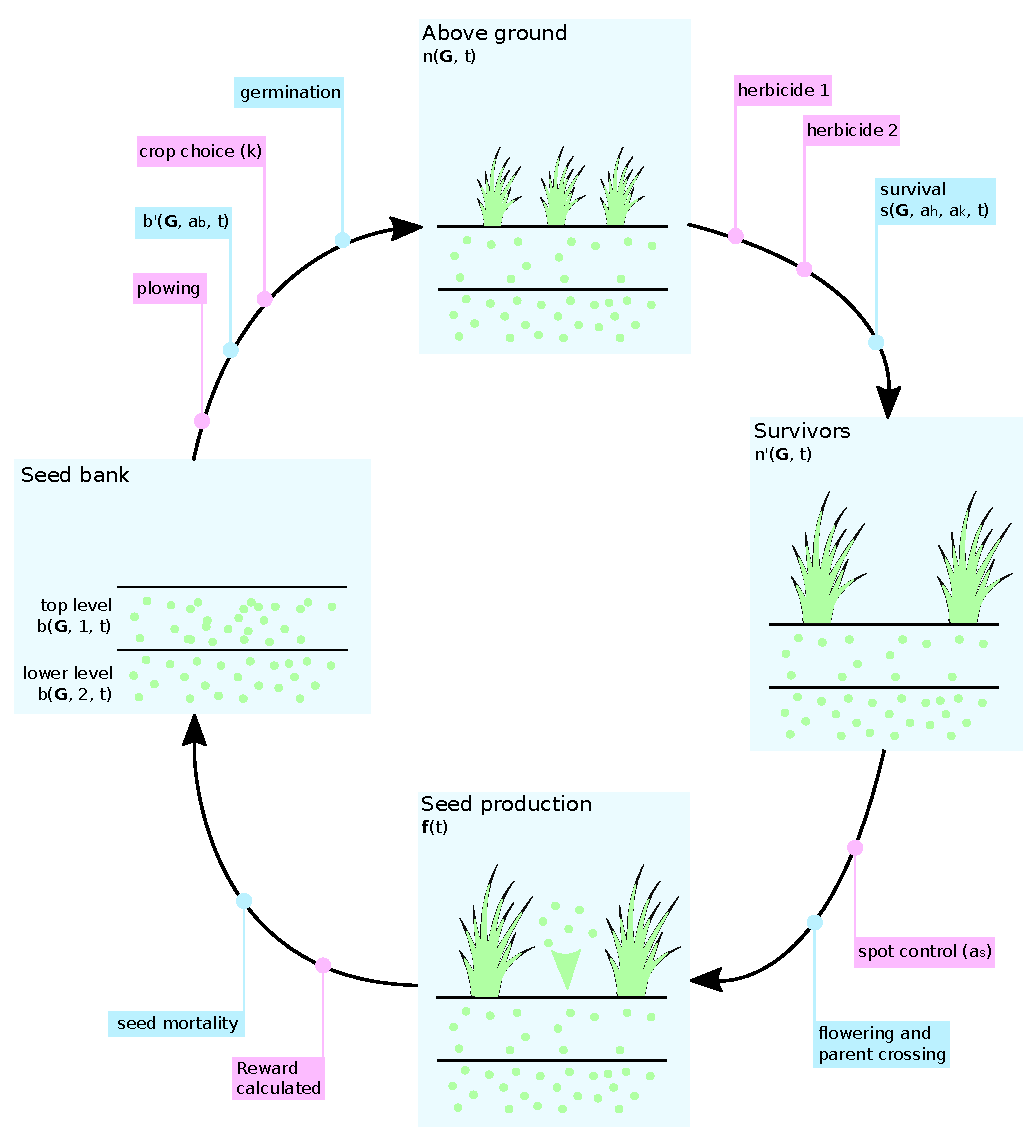
\includegraphics[scale=0.7]{/home/shauncoutts/Dropbox/projects/MHR_blackgrass/IWM_optimisation/writting/figures/pop_mod_2sb_scheme.pdf}
\caption{Life cycle with management interventions over the year. Pink processes are management interventions and blue processes are biological population processes.}
\label{fig:life_cyc}
\end{figure} 

Finally new seeds are created from these parent distributions by mixing simultaneously over both $g_1$ and $g_2$. The number of seeds produced with resistance $g_1$ and $g_2$ at time $t$ is 
\begin{equation}
\label{eq:fec}
\begin{split}
	f(g_1, g_2, t) = \int_{g_1^m}\int_{g_1^p}\int_{g_2^m}\int_{g_2^p} n'''(g_1^m, g_2^m, t)f_{max} \frac{n'''(g_1^p, g_2^p, t)}{N'''(t)}MV&N(g_1, g_2| \mathbf{\mu}, \mathbf{\Sigma})\cdot\\ &\text{d}g_1^m\text{d}g_1^p\text{d}g_2^m\text{d}g_2^p
\end{split}	
\end{equation} 
where $g_j^m$ is resistance trait $j$ of the maternal parent and $g_j^p$ is resistance trait $j$ of the paternal parent and, $n'''(g_1, g_2, t)$ is defined in Eq. \ref{eq:eff_pop}. We assume that pollen is never limiting, and so only the relative frequency of the paternal resistance $(g_1^p, g_2^p)$ is important, thus we divide effective reproductive population $n'''(g_1^p, g_2^p, t)$ by
\begin{equation}\label{eq:tot_pop3}
	N'''(t) = \int_{g_1}\int_{g_2} n'''(g_1, g_2, t) \text{d}g_1\text{d}g_2 
\end{equation}  
to create a probability distribution. The probability of an offspring with resistance $(g_1, g_2)$ being produced by parents with resistance $(g_1^m, g_2^m)$ and $(g_1^p, g_2^p)$ is $MVN(g_1, g_2| \mathbf{\mu}, \mathbf{\Sigma})$. The offspring distribution is assumed to be multivariate normal, $MVN(\cdot)$, over breeding values $(g_1, g_2)$, with a mean of vector
\begin{equation*}
	\mathbf{\mu} = \begin{bmatrix}
		\frac{g_1^m + g_1^p}{2}\\
		\frac{g_2^m + g_2^p}{2}
		\end{bmatrix}   
\end{equation*}
and covariance matrix $\mathbf{\Sigma}$, which encodes both the variance of the offspring distribution and the covariance in inheritance of traits $(g_1, g_2)$. We start with the simplest case and assume that the variance in the breeding value of offspring is the same for both $g_1$ and $g_2$, and that there is no covariance in their inheritance (i.e. traits $g_1$ and $g_2$ are inherited independently). These assumptions give the covariance matrix    
\begin{equation}
	\mathbf{\Sigma} = \begin{bmatrix}
		\sigma_f & 0\\
		0 & \sigma_f
	\end{bmatrix}
\end{equation}
where $\sigma$ is assumed to be twice the additive variance (i.e. $\sigma = 2V_A$). Finally, $f_{max}$ is the number of seeds produced by an individual that is susceptible to both herbicides at low densities.   

\subsection*{Management strategy}
Our goal is to find good strategists to manage black grass in the face of evolving resistance, however it is not feasible to test every combination of management options over more than a handful of years. Even in our simplified action space there are 34 combinations of sub-actions, and over 10 years there are approx 2.064$\times 10^{15}$ possible sequences of actions. Finding the optimal sequence of actions among this large number of possibilities is a combinatorial optimization problem, one of the hardest classes of problems to solve (NP-hard). However, genetic algorithms have been used to find good solutions to this class of problem [REF]. The genetic algorithm starts with an randomly generated set of action sequence, these action sequences are then iteratively improved to find a set of good action sequences. Genetic algorithms rely on the fact that even though the number of possible action sequences is large many of these will perform very poorly. The genetic algorithm explores better performing regions of the solution space explored more intensely (avoiding the poor performing regions). While genetic algorithms are not guaranteed to find the optimal action sequence they will find a set of actions sequences that perform well, often close to the optimal solution.   

The first step in finding good action sequences is defining a reward function that encodes the goals of a manager [REF]. We assume farmers are primarily driven by economic returns. The economic return consists of two parts, the income made from the crop and the costs of producing that crop. We assume that usual farm costs, such as buildings and machinery as constant from year to year, so we focus on gross margin, i.e. income - variable costs [NIX2017].

Income from the crop in year $t$ is    
\begin{equation}\label{eq:yield}
	Y(N'', a_k^t, a_k^{t-1}) = \begin{cases} 
		W(a_k^t, a_k^{t-1})(Y_0 - \beta_D N')P &~\text{if}~a_k^t = \text{wheat}\\
		W(a_k^t, a_k^{t-1})\vartheta &~\text{if}~a_k^t = \text{alt}\\
		0 &~\text{if}~a_k^t = \text{fallow}\\
	\end{cases}
\end{equation}   
where $Y_0$ is the yield of winter wheat (in t/ha) when the density of black grass after management ($N''$) is 0, $\beta_D$ is the rate at which yield decreases with increasing black grass density and $P$ is the price of winter wheat, taken from [NIX2017] as £146/t. Yield of a crop can be affected by planting the same crop two years in a row, largely due to species specific parasites and pathogens in the soil [REF Kwadjo]. We use the weighting function 
\begin{equation}
	W(a_k^t, a_k^{t-1}) = \begin{cases}
		\varpi &~\text{if}~a_k^t = a_k^{t-1}\\
		1 &~\text{otherwise}
	\end{cases}
\end{equation} 
to reduce yield if the same crop is used two times in succession, where $\varpi \in [0, 1]$ is the proportional yield achieved when the same crop is used, following [REF Kwadjo] we use $\varpi = 0.9$. We assume the yield of the alternative crop, $\varphi$, is not affected by black grass. The alternative crop is based on spring barley, a common spring crop used in the UK for the control of black grass. The average income from spring barley is \pounds 796/ha [NIX2017 pp ??].   

Costs depend on both the action chosen and non-weed control costs, such as fertilizer, seed and other sprays such as fungicides. We assume these other variable costs change with crop choice ($a_k$), but are constant from year to year within a crop choice. Thus the cost of action is $a_q$  
\begin{equation}
	C(a_q^t) = \sum_{\forall a_s \in a_q^t} c(a_s)
\end{equation}
where $c(a_s)$ is the cost of sub-action $a_s$. 

The cost for herbicide action $a_h$ is  
\begin{equation}\label{eq:herb_cost}
	c(a_h) = \begin{cases}
		0~&\text{if}~a_h = 0\\
		\theta_h~&\text{if}~a_h = 1 \bigvee a_h = 2 \\
		2\theta_h~&\text{if}~a_h = \text{both}
	\end{cases}
\end{equation}
Where $\theta_h$ is the cost of a single herbicide application to control black grass. We assume that most herbicide costs in winter wheat are associated with black grass control, and so take $\theta_h = \pounds 96$ [REF NIX2017 pp. ??]. 

The cost function crop choice is 
\begin{equation}\label{eq:crop_cost}
	c(a_k) = \theta_{a_k}
\end{equation}   
where the parameter $\theta_{a_k}$ are the constant costs not associated with each crop choice. The cost for winter wheat excludes herbicide costs associated with black grass control, and is taken as $\theta_\text{wheat} = $\pounds 383/ha [NIX2017 pp??]. We assume both a fallow rotation and the alternative crop are used, at least in part, to control black grass, and so we include all costs, including those associated with black grass control in $\theta_\text{alt} = $\pounds 273/ha [NIX2017 pp??] and $\theta_\text{fallow} = $ \pounds 36/ha [NIX2017 pp. 202 and 284]. The cost of the fallow rotation is based on two applications of glyphosate (a broad spectrum herbicide) to kill back grass after it has germinated.       

The cost function for plowing is 
\begin{equation}\label{eq:plow_cost}
	c(a_b) = \theta_b a_b 
\end{equation}
where $\theta_b = $ \pounds 73.96/ha is the contractor rates for deep plowing (which are assumed to combine all labour and capital costs) [Nix2017 pp. 202], and $a_b \in \{0, 1\}$. 

Finally the cost function for spot control is assumed to increase proportionally with black grass density after other control actions have been taken ($N'$) so that
\begin{equation}
	c(a_m, N', N'', a_k^t, a_k^{t-1}) = \textbf{min}\left( Y(N'', a_k^t, a_k^{t-1}),~ Y(N'', a_k^t, a_k^{t-1})\delta N' (1 - a_m) \right)
\end{equation}  
where $\delta$ controls how quickly the costs of spot control increase with black grass density. We assume that spot control also kills all the crop in a controlled area, for example patch spraying a high density infestation with a broad spectrum herbicide. we assume our field is 1 ha in size and that high density black grass infestations are 9.6666 plants/m$^2$ [REF Queenborough et al 2010]. Thus, if the whole hectare was at high density there would be 96666 plants. We assume one would have to kill the entire crop to control such a population with spot control. Further, we assume crop loss is the main cost for spot control and that the relationship between crop loss and black grass population is linear. Under these assumptions $\delta = 1/96666$. $Y(N'', a_k^t, a_k^{t-1})$ is the income for the crop choice in time $t$ and (Eq. \ref{eq:yield}) and scales the cost to the income that would have been generated if part of the crop did not have to be destroyed. $a_m \in \{0, 1\}$ is a switch, also used in Eq. \ref{eq:spot_cont}), that is 0 if spot control is done.        

The economic reward is a function of $N''$, the total above ground population size after management had been carried out (defined in Eq. \ref{eq:tot_pop2}). To explicitly link the above ground population to the reward function we define $N''(\mathbf{a}, n_0, t)$, the total above ground population after all control actions, at time $t$ given an initial population $n_0$ and a sequence of actions 
\begin{equation}
	\mathbf{a} = \{a_q^1, a_q^2, \cdots, a_q^T\}
\end{equation}	   
where $a_q^t$ is the action $a_q \in \mathbf{A}$ taken at time $t$ and $T$ is the time horizon over which management is run. We assume all returns after $T$ are ignored. The reward function is  
\begin{equation}
	R(\mathbf{a}, n_0) = \sum_{t=0}^T \gamma^t \Big( Y(N'(\mathbf{a}, n_0, t)) - C(a_k^t) \Big)
\end{equation}
where $R(\mathbf{a}, n_0)$ is the time discounted reward for action sequence $\mathbf{a}$ given starting population $n_0$, $\gamma \in [0, 1]$ is the discount rate. When $\gamma = 0$ only the reward in the first time step is considered, when $\gamma = 1$ returns in all future time steps are valued equally.

To find good action sequences we use a genetic algorithm with knock out tournament selection, where each action sequence is randomly paired with another, and the action sequence with the highest $R(\mathbf{a}, n_0)$ survives to help generate new action sequences. We used pair mating between survivors and N-point cross-over to produce new action sequences. After new action sequences are created there is a process of random mutation where each $a_q^t$ is changed to another $a_q^t \in \mathbf{A}$ with probability $m$. The algorithm used is given in Appendix 2.        

\subsection*{parametrization of yield function}
To fit the yield function in Eq. \ref{eq:yield} we use data from 10 fields where harvesters recorded wheat yield for every 20m by 20m gird square of the field. We also have black grass density estimates for each grid square from state structured surveys [REF audit paper]. These density states were calibrated to plants/m$^2$ by [REF Queenborough et al 2010]: the density states were absent (0 [0--0.1667] plants/m$^2$)(median[inter-quartile range]), low (0.5000 [0.1667--1.5000] plants/m$^2$), medium (2.6666 [1.3333--4.7500] plants/m$^2$), high (5.0833 [3.0000--7.7916] plants/m$^2$), and very high (9.6666 [7.1250--13.1666] plants/m$^2$). We fit a linear yield function 
\begin{subequations}
\label{eq:est_yield}
\begin{equation}
 Y_i \sim N(\widehat{Y_i}, \sigma_y)
\end{equation}
\begin{equation}
	\widehat{Y_i} = Y_0 + Y_0^j + (\beta_D + \beta_D^j)D 
\end{equation}
\end{subequations}
We assume the yield for grid square $i$ ($Y_i$, in t/ha) is drawn from a normal distribution with standard deviation $\sigma_y$. Predicted yield ($\widehat{Y_i}$) is a linear function of black grass density, where $Y_0$ is the average winter wheat yield across all fields and $Y_0^j \sim N(0, \sigma_y^0)$ is the random effect of field $j$ on the intercept of field, drawn from a normal distribution with mean of 0 and standard deviation of $\sigma_y^0$. $\beta_D$ is the change in yield when black grass density ($D$) changes by 1 plant/$m^2$, averaged across all fields, and $\beta_D^j \sim N(0, \sigma_y^D)$ is the effect of field on the relationship between black grass density and yield. This model was fit with the 'lme4' package [REF] in the R statistical language [REF]. We are interested in the average yield loss and so the yield function in Eq. \ref{eq:yield} is $Y_0 + \beta_D N''$. We assume our population exists in a 1ha field. Converting from plants/m$^2$ to plants/ha the yield loss function becomes 
\begin{equation}
	\widehat{Y} = 11.43 - 0.0000223 N'' 
\end{equation}
All costs are \pounds, to put the yield and costs on the same scale we assume a winter wheat price of \pounds 146/t [NIX 2017], 
\begin{equation}
	\widehat{Y} = 1668 - 0.00326 N'' 
\end{equation}


\newpage
\section*{Appendix 1: Action space}
\begin{longtable}[h]{c p{9cm} p{4cm}}
\caption{Management sub-actions and their effects on the population model\label{table:actions}}\\
	\hline
	\textbf{Sub-action} & \textbf{Effect on system model} & \textbf{Management parameters}\\
	\hline	
	\multicolumn{3}{l}{\textit{Crop choice}: $a_k$, levels 1 -- 3}\\
	wheat & higher survival rate for black grass and herbicide less effective due to spraying occurring earlier & Highest profit in the absence of black grass \\
	alt & Black grass survival reduced under alternative crop due to competition or broad spectrum herbicide use before sowing & lower income than wheat\\
	fallow & no crop planted. All above ground plants killed as we assume used alongside plowing or broad spectrum herbicide & small negative income, no production, costs for killing above ground plants\\
	\multicolumn{3}{l}{\textit{Herbicide}: $a_h$, levels 1 -- 4}\\
	no herb & no effect & no cost\\ 
	herb 1 & reduced survival for emerged individuals with low $g_1$, high $g_2$ level may provide some protection if there is cross resistance. & small application cost.\\
	herb 2 & reduced survival for emerged individuals with low $g_2$, high $g_1$ level may provide some protection if there is cross resistance. & small application cost.\\  
	both & reduced survival for emerged individuals with low $g_2$ or $g_1$. & larger application cost.\\  
	\multicolumn{3}{l}{\textit{Seed bank management}: $a_b$, levels 1 -- 2}\\
	1 & Moves seeds from one level of the seed bank to the other & fixed cost\\
	0 & no effect & no cost\\
	\multicolumn{3}{l}{\textit{spot control}: $a_m$, levels 1 -- 2}\\
	1 & No effect of above ground population & No cost\\
	0 & Kills all remaining above ground plants & Cost scales with above ground post control populations $N'$ (Eq. \ref{eq:tot_pop1} \\
	\hline
\end{longtable}

\newpage
These sub-actions are combined to create a single action $a_q$ that could be taken in a time step. However some sub-action combinations do not make sense, for example applying herbicide to the population when $a_k =$ 'fallow', since we assume all above ground plants are destroyed under this crop choice. The list of all allowed sub-action combinations is the action space $\mathbf{A}$   

\begin{longtable}[h]{c c c c c c}
\caption{Action space ($\mathbf{A}$) with all eligable combinations of sub actions\label{table:action_space}}\\
	\hline
	$\mathbf{a_q}$ & $\mathbf{a_k}$ & $\mathbf{a_h}$ & $\mathbf{a_b}$ & $\mathbf{a_m}$\\
	\hline
	$a_1$ & wheat & no herb & 0 & 1\\
	$a_2$ & wheat & no herb & 0 & 0\\
	$a_3$ & wheat & no herb & 1 & 1\\
	$a_4$ & wheat & no herb & 1 & 0\\
	$a_5$ & wheat & herb 1 & 0 & 1\\
	$a_6$ & wheat & herb 1 & 0 & 0\\
	$a_7$ & wheat & herb 1 & 1 & 1\\
	$a_8$ & wheat & herb 1 & 1 & 0\\
	$a_9$ & wheat & herb 2 & 0 & 1\\
	$a_{10}$ & wheat & herb 2 & 0 & 0\\
	$a_{11}$ & wheat & herb 2 & 1 & 1\\
	$a_{12}$ & wheat & herb 2 & 1 & 0\\
	$a_{13}$ & wheat & both & 0 & 1\\
	$a_{14}$ & wheat & both & 0 & 0\\
	$a_{15}$ & wheat & both & 1 & 1\\
	$a_{16}$ & wheat & both & 1 & 0\\
	$a_{17}$ & alt & no herb & 0 & 1\\
	$a_{18}$ & alt & no herb & 0 & 0\\
	$a_{19}$ & alt & no herb & 1 & 1\\
	$a_{20}$ & alt & no herb & 1 & 0\\
	$a_{21}$ & alt & herb 1 & 0 & 1\\
	$a_{22}$ & alt & herb 1 & 0 & 0\\
	$a_{23}$ & alt & herb 1 & 1 & 1\\
	$a_{24}$ & alt & herb 1 & 1 & 0\\
	$a_{25}$ & alt & herb 2 & 0 & 1\\
	$a_{26}$ & alt & herb 2 & 0 & 0\\
	$a_{27}$ & alt & herb 2 & 1 & 1\\
	$a_{28}$ & alt & herb 2 & 1 & 0\\
	$a_{29}$ & alt & both & 0 & 1\\
	$a_{30}$ & alt & both & 0 & 0\\
	$a_{31}$ & alt & both & 1 & 1\\
	$a_{32}$ & alt & both & 1 & 0\\
	$a_{33}$ & fallow & no herb & 0 & 1\\
	$a_{34}$ & fallow & no herb & 1 & 1\\
	\hline
\end{longtable}

\section*{Appendix 2}
{\setstretch{1.0}
\begin{algorithm}[H]
\caption{Genetic algorithm used to find good sequences of management actions}
\label{alg:HDP}
\begin{algorithmic}[1]
	\For{rep = 1 \textbf{to} rep = number\_reps}	
		\State Randomly generate initial population $P$ of action sequences $\textbf{a}$.
		\For{gen = 1 \textbf{to} gen = number\_gen}
			\ForAll{$\textbf{a} \in P$}
				\State Initialize population in state $n_0$
				\For{$t = 1~\textbf{to}~t = T$} 
					\State Run the population model under action sequence $\textbf{a}$ 
					\State Record $N''(\mathbf{a}, n_0, t)$ at each step.
				\EndFor
				\State Calculate $R(\mathbf{a}, n_0)$
			\EndFor
			\State Randomly pair each $\textbf{a} \in P$
			\State For each pair put the $\textbf{a}$ with the highest $R(\mathbf{a}, n_0)$ into population  $P'$.
			\State Randomly pair each $\textbf{a} \in P'$
			\ForAll{pairs}
				\State Copy each sequence in the pair to $\textbf{a}_1^*$ and $\textbf{a}_2^*$ 
				\State Randomly select a point $t^* \in 2:(T - 1)$
				\State Swap section $\textbf{a}_1^*[1:t^*]$ and $\textbf{a}_2^*[1:t^*]$
				\State $\forall a^t \in \textbf{a}_j^*$, $a^t \gets a^{t*} \in \textbf{A}$ with probability $m$  
				\State Put $\textbf{a}_j^*$ into $P'$.   
			\EndFor
			\State $P \gets P'$    
		\EndFor	 
	\EndFor
	\State Compare $\textbf{a}$ with highest $R(\mathbf{a}, n_0)$ from each $P$ in the final generation between reps to check they have converged on the same action sequence.   
\end{algorithmic}
\end{algorithm}  
}


\end{document}